% Thesis subsection: boundary behaviour of CBO-U interventions.
% Requires in the main preamble: \usepackage{graphicx,booktabs,amsmath}
% Set the graphics path to where the figures live, e.g.
%   \graphicspath{{results/boundary_tracking/plots/}}

\subsection{Boundary behaviour of CBO-U interventions}
\label{sec:boundary-behaviour}

For a noiseless linear SEM the causal effect of a genuine parent on the target is monotonic, so the value-minimising intervention on that parent sits at an \emph{extreme} of its allowed range. We therefore expect CBO-U (the \texttt{PARENT\_SCALE} doubly-robust variant) to exhibit a \emph{boundary bias} in the intervention values it selects, and to retain it as graphs grow. The observation motivating this section is that on large graphs (Erdos100) the interventions did \emph{not} appear to hug the boundary, and the parent posterior was simultaneously inaccurate. We ask: (i) is there a boundary bias at all, and does it hold at scale; and (ii) is the inaccurate posterior related to it?

All runs use \texttt{PARENT\_SCALE} (CBO-U, \texttt{dr2}, \texttt{individual=True}) on noiseless linear Erdos--R\'enyi SEMs, with $n_{\text{obs}}=200$, $30$ trials, seed $71$, for three sizes: Erdos20 (true parents $\{4\}$), Erdos50 ($\{19,49\}$) and Erdos100 ($\{85,98\}$). We test the boundary question directly from the recorded intervention values: for each intervened dimension we compute its normalised position in the variable's range,
%
\begin{equation}
  p \;=\; \frac{\text{value} - \text{lower}}{\text{upper} - \text{lower}} \;\in\; [0,1],
  \qquad d \;=\; \min(p,\,1-p),
\end{equation}
%
where $d$ is the distance to the nearest edge. Under a uniform null (values drawn at random from the range) the deciles of $p$ are flat, $\mathbb{E}[d]=0.25$, and the fraction of interventions in the outer-$20\%$ edge zones ($p<0.2$ or $p>0.8$) is $40\%$. We compare against this null with a one-sided binomial test on the outer-band count.

\subsubsection{A boundary bias exists, but only on true parents}

Splitting every intervention by whether the intervened variable is an actual parent of the target gives a clean separation (Fig.~\ref{fig:bias-by-parent}). True-parent interventions (pooled, $n=60$) have mean position $0.13$, with $82\%$ in the outer-$20\%$ edge zones versus the $40\%$ null ($p = 4.6\times10^{-11}$) and mean distance-to-edge $0.10$; they pile up at the \emph{lower} edge, consistent with pushing a monotone parent down to minimise the target. Non-parent interventions ($n=30$, all from Erdos100) have mean position $0.48$, only $3\%$ in the edge zones, and mean distance-to-edge $0.35$; they sit in the \emph{centre}. The boundary bias is thus real and highly significant, but conditional on intervening on a variable that genuinely drives the target.

\begin{figure}[htbp]
  \centering
  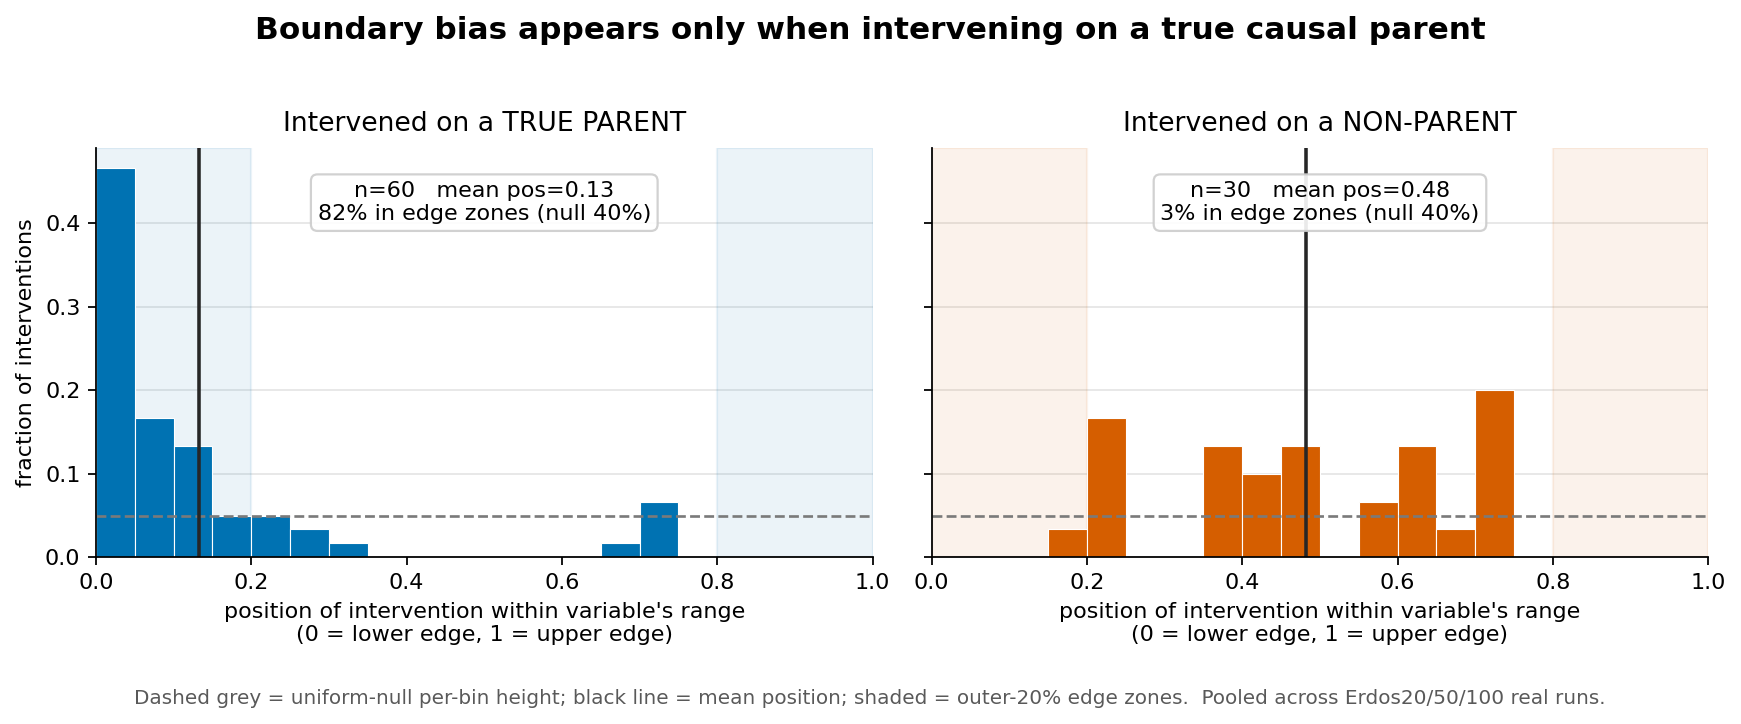
\includegraphics[width=\linewidth]{fig1_boundary_bias_by_parent.png}
  \caption{Pooled distribution of the normalised intervention position $p$, split by whether the intervened variable is a true parent. True-parent interventions concentrate at the lower edge ($82\%$ in the edge zones); non-parent interventions sit in the centre ($3\%$). Dashed line: uniform null per-bin height; vertical line: mean position; shaded: outer-$20\%$ edge zones.}
  \label{fig:bias-by-parent}
\end{figure}

\subsubsection{The posterior collapses onto the wrong variables, worst at scale}

Diagnostics on the recorded posteriors show that for larger graphs the exploration set collapses --- at iteration $0$, before any CBO trial --- onto too few and often wrong candidate parents. Erdos20 recovers $\{4\}$ correctly; Erdos50 collapses to $\{49\}$, dropping the true parent $19$; and Erdos100 collapses to a non-parent ($\{90\}$/$\{64\}$), with neither true parent present from iteration $0$ onward. Because the candidate set can only shrink after iteration $0$ (hypotheses are deleted, never re-added), a true parent missing at the cold start is locked out for the entire run, so Erdos100 spent all $30$ trials intervening on non-causal variables.

Isolating the cold-start step shows the doubly-robust bootstrap is not the whole story: $8$ of $10$ bootstrap draws on Erdos50 do contain both true parents $\{19,49\}$, but nearly every draw also adds false positives, so the exact true set receives only $20\%$ of the mass, and the subsequent Bayesian update from the initial interventional data collapses this to the single wrong-ish $\{49\}$. The root cause of the inaccurate posterior is therefore false-positive-heavy parent identification together with an over-aggressive initial collapse, amplified as the candidate pool grows with graph size.

\subsubsection{Confound-closing experiment: fixing the parents flips centre to edge}

The two findings above suggest that the absence of boundary bias on Erdos100 is a \emph{consequence} of intervening on non-parents, not a failure of the boundary mechanism at scale. However, in the real runs ``true parent'' is confounded with ``small/medium graph''. To break the confound we re-ran Erdos50 and Erdos100 with an \emph{oracle}: the parent posterior is forced to the true parent set (probability $1.0$), bypassing the bootstrap, while the acquisition, the GP surrogates and the boundary tracking are otherwise identical. On the same $100$-node graph, forcing the true parents flips the behaviour completely (Table~\ref{tab:confound}, Fig.~\ref{fig:confound}): the strict boundary percentage rises from $0.00$ to $0.47$, and $26$ of $30$ interventions land in the lowest decile of the range. The Erdos50 oracle is a positive control and stays edge-biased ($73\%$).

\begin{table}[htbp]
  \centering
  \begin{tabular}{lcccc}
    \toprule
    Erdos100 & intervenes on & outer-$20\%$ band & mean position & verdict \\
    \midrule
    Real   & non-parents $90,64$  & $3\%$   & $0.48$ & no bias (centre) \\
    Oracle & true parents $85,98$ & $90\%$  & $0.06$ & strong edge bias \\
    \bottomrule
  \end{tabular}
  \caption{The same $100$-node graph under the real (collapsed) posterior versus the oracle (true parents forced). Only the selected variables differ.}
  \label{tab:confound}
\end{table}

\begin{figure}[htbp]
  \centering
  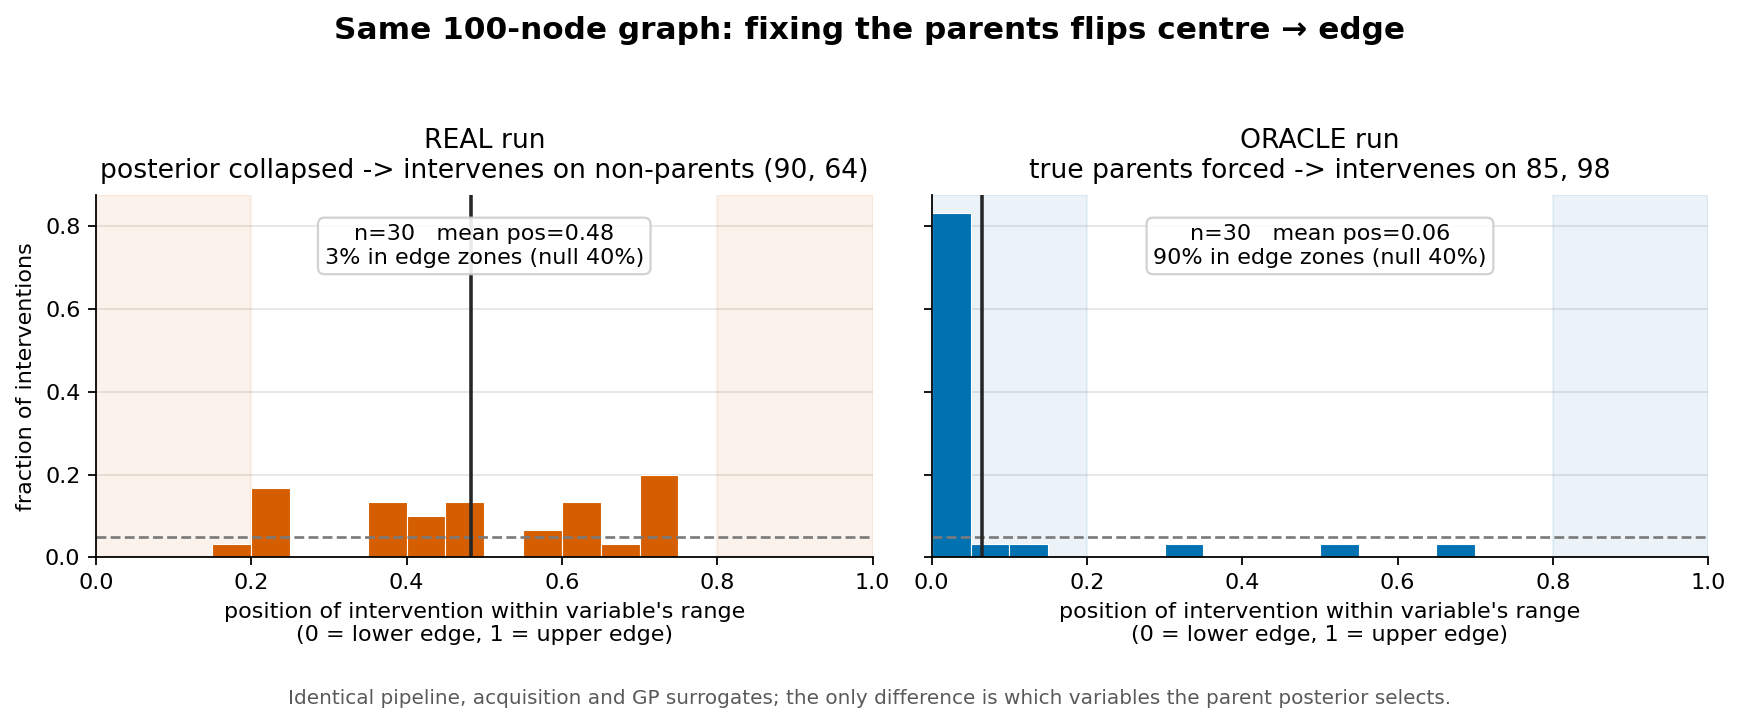
\includegraphics[width=\linewidth]{fig2_confound_erdos100_real_vs_oracle.png}
  \caption{Erdos100, real versus oracle. Identical pipeline, acquisition and GP surrogates; the only difference is which variables the parent posterior selects. The real run intervenes on non-parents and sits in the centre; the oracle run intervenes on the true parents and hugs the edge.}
  \label{fig:confound}
\end{figure}

Across all runs (Fig.~\ref{fig:summary}), every run that intervenes on true parents --- regardless of graph size --- is far above the $40\%$ null; the sole exception is Erdos100-real, which fails only because it selected the wrong variables. Erdos100-oracle, immediately beside it, reaches $90\%$.

\begin{figure}[htbp]
  \centering
  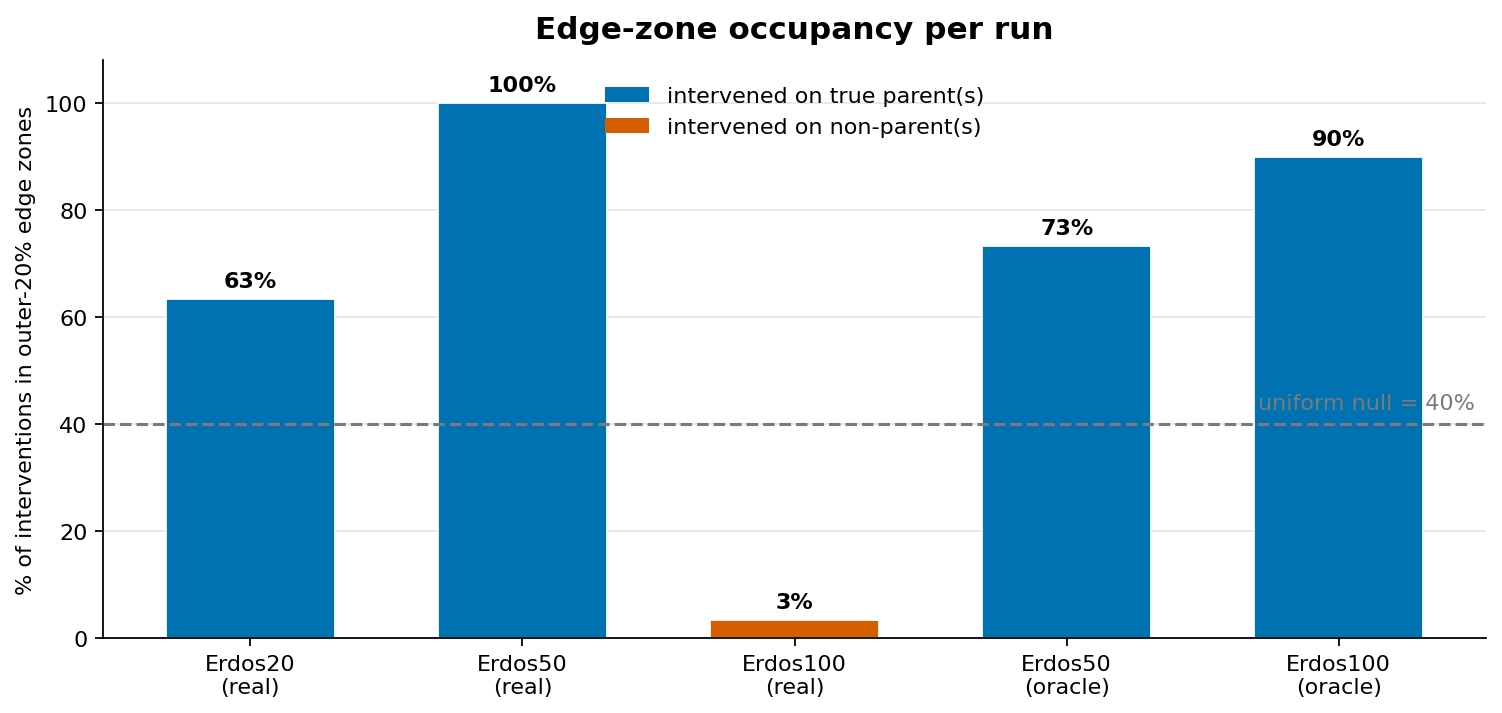
\includegraphics[width=0.85\linewidth]{fig3_summary_outer_band.png}
  \caption{Fraction of interventions in the outer-$20\%$ edge zones per run, against the $40\%$ uniform null. Blue: intervened on true parents; orange: intervened on non-parents.}
  \label{fig:summary}
\end{figure}

\subsubsection{Why a non-parent produces no boundary behaviour}

This follows from the surrogate construction. The acquisition's GP prior mean is the do-effect $\mathbb{E}[Y\mid \mathrm{do}(X=x)]$, computed by propagating the intervention through the fitted SEM (\texttt{causal\_effect\_DO}). For a hypothesised parent, the target is regressed on that variable from observational data (\texttt{functions[target]}). When the hypothesis is wrong the variable carries no information about the target, so this regression has approximately zero slope and the do-effect surface is flat,
%
\begin{equation}
  \mathbb{E}[Y \mid \mathrm{do}(90 = x)]
  \;=\; \texttt{functions[target]}.\text{predict}(90=x)
  \;\approx\; \mathbb{E}[Y] \quad \text{for all } x .
\end{equation}
%
The flatness is not incidental: it is the same fact as the parent being wrong, since the model regresses the target on a variable that does not explain it. A flat surface gives the optimiser no gradient toward either edge, so the intervention settles in the data-dense centre (the observational mean, where the GP is best determined) rather than extrapolating to the sparse range extremes. A true parent gives a real slope, hence a monotone surface whose optimum sits at the edge --- exactly as observed, with non-parent interventions landing at the variable's observational mean ($p\approx0.5$) and true parents at the edge ($p\approx0.05$).

\subsubsection{Conclusion}

There is a genuine boundary bias, and it works at scale: a $100$-node graph hugs the boundary as strongly as a $50$-node one when it intervenes on the true parents ($90\%$ versus $73\%$). The two symptoms are one root cause --- the inaccurate posterior makes the algorithm intervene on non-causal variables, which produce flat do-effect surfaces with no boundary optimum, so the apparent loss of boundary-seeking at scale is entirely downstream of the parent-identification failure. The fix is therefore upstream: the boundary behaviour needs no change and follows automatically once the true parents survive into the exploration set, which calls for reducing the bootstrap's false-positive rate, softening the initial interventional collapse that drops true parents, and seeding the bootstrap resampling.

Two caveats bound these conclusions. The runs use a single seed per graph, so a few additional oracle seeds on Erdos100 would confirm the $90\%$ is not seed-specific (cheap, since the oracle skips the bootstrap). And the true-parent/non-parent split in Fig.~\ref{fig:bias-by-parent} is itself confounded with graph size in the real data; the confound-closing claim rests on the oracle experiment (Fig.~\ref{fig:confound}), not on Fig.~\ref{fig:bias-by-parent}.
